\documentclass{main}
\begin{document}
\section{Tor - Onion Routing}
Tor has been one of the most famous and widely used anonymous communication tool.
Tor, The onion Routing Browser is simply an Internet Browser based on Firefox, with modifications to hide the user's IP address. 
Although Tor was initially developed by the US government in 2002, it is not presently controlled by any one entity.

\subsection{Onion Routing}

\begin{wrapfigure}{l}{0.6\textwidth}
    \centering
    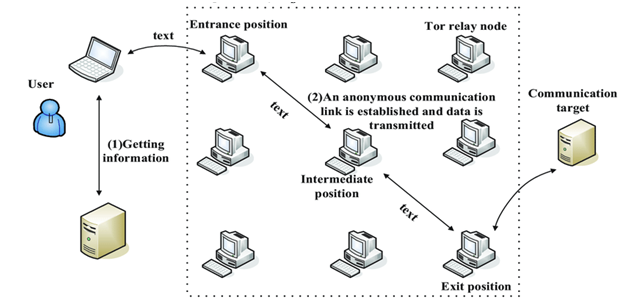
\includegraphics[width=0.6\textwidth]{Resources/images/onion-routing.png}
\end{wrapfigure}

In a nutshell, onion routing refers to encapsulating message under layers of encryption at different nodes before it reaches the final destination. 
All the nodes only know about the previous node and the next node. 
In this way, no single node knows the entire path of the message. 
Clients choose these path randomly and build a circuit. 
These circuits change every few minutes preventing any snooping attempts. 







\end{document}
